\section{Doménový model}
Doménový model (na obrázku \emph{\ref{diagram-domenovy}} a \emph{\ref{diagram-domenovy-brickset}}) popisuje strukturu dat a vazby mezi jednotlivými entitami. Je důležitý pro učinění rozhodnutí jaké objekty a jejich vztahy bude nutné v aplikaci uchovávat. 

Při vytváření doménového modelu je vycházeno ze tří zdrojů dat, které jsou stanoveny v rešeršní části práce. Z hlediska domény je tedy vhodné rozdělit entity do balíčků podle zdroje, ze kterého pochází. Využité zdroje dat jsou: 
\begin{itemize}
  \item knihovna LDraw,
  \item Rebrickable,
  \item Brickset.
\end{itemize}

Pro větší přehlednost jsem doménový model rozdělil na dva diagramy. Diagram na obrázku \ref{diagram-domenovy} popisuje lokálně ukládaná data knihovny LDraw a služy Rebrickable. Diagram na obrázku \ref{diagram-domenovy-brickset} data dostupná přes API Brickset. 

\begin{figure}[htbp]
    \centering
    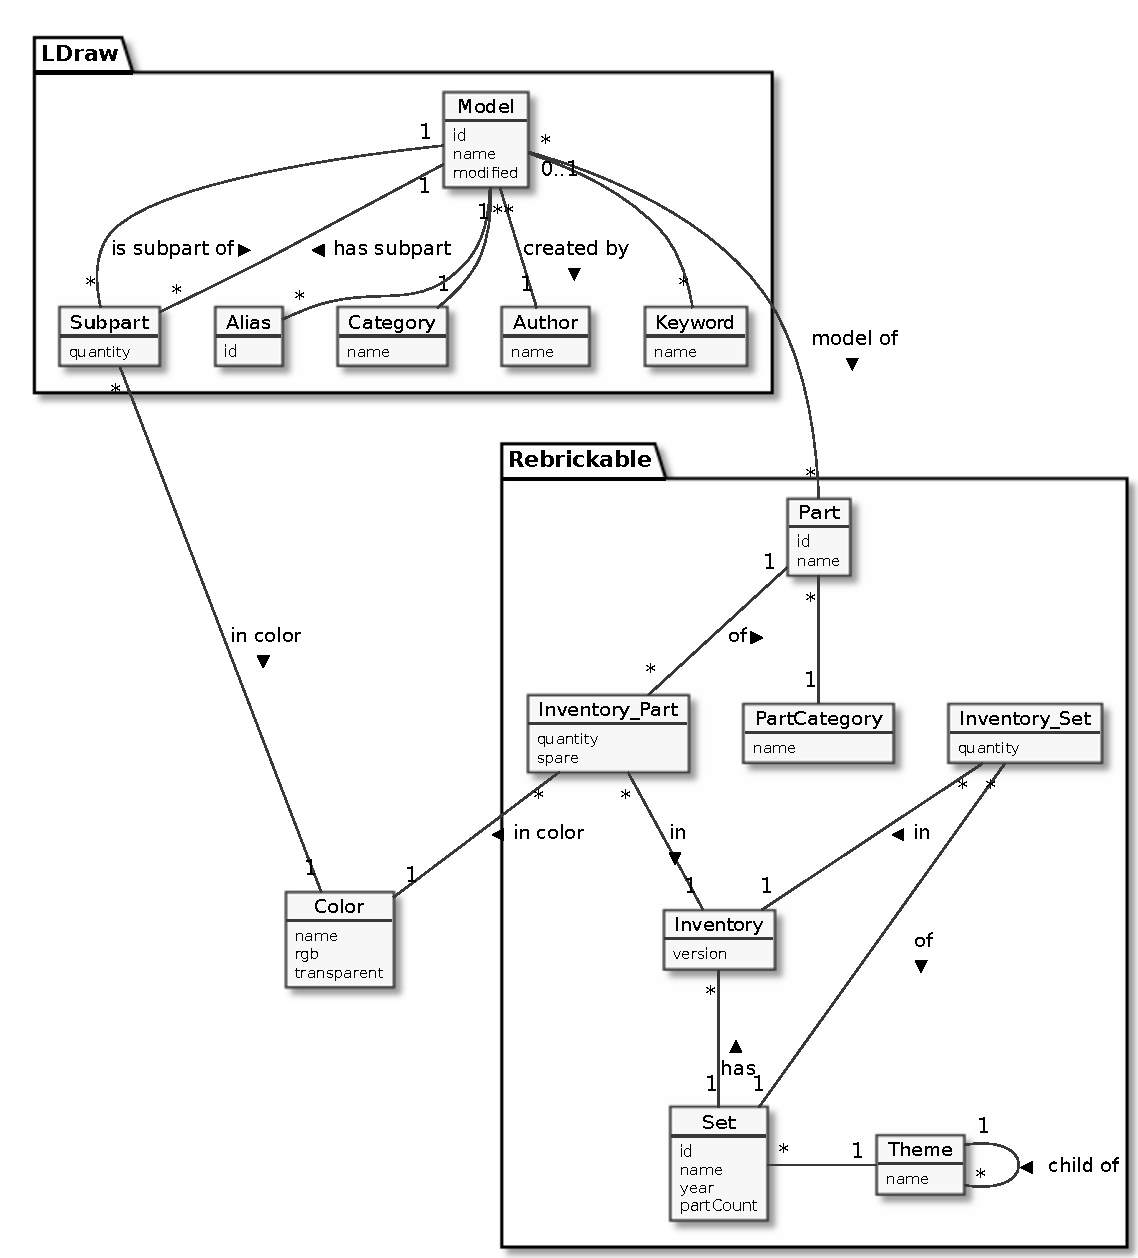
\includegraphics[width=\textwidth,height=\textheight,keepaspectratio]{pdfs/domain_ldraw_rebrickable}
    \caption{Doménový model: LDrawkey a Rebrickable\label{diagram-domenovy}}
  \end{figure}

\subsection{LDraw}
První balíček obsauje entity týkající se součástek z knihovny LDraw.

\subsubsection*{Model}
  Entita \textit{Model} (tabulka \emph{\ref{table:entity:model}}) reprezentuje jednu součástku z knihovny LDraw. Atributy entity vychází z dat obsažených v jednotlivých souborech knihovny a ze specifikace hlavičky, která byla představena v podsekci \emph{\nameref{ldraw-hlavicka}} sekce \ref{reserse-ldraw}.
    
  U každého \textit{Modelu} musí být evidován jeho autor z důvodu možnosti dodržení licence \gls{CC-BY} \cite{CC-BY}, pod kterou jsou zveřejněny všechny součástky v oficiální knihovně LDraw. 
  
  \begin{table}[th!]
  \centering
  \caption{Přehled atributů entity \textit{Model}}
  \label{table:entity:model}
  \begin{tabularx}{\textwidth}{@{}rX@{}}
  \toprule
  Atribut & Popis
  \\ 
  \midrule
  id: & Unikátní textový identifikátor modelu
  \\
  name: & Jméno modelu 
  \\
  modified: & Datum poslední úpravy modelu 
  \\
  partCount: & Počet součástek ve stavebnici
  \\
  path: & Cesta k souboru 3D modelu na serveru
  \\
  \bottomrule
  \end{tabularx}
  \end{table}

\subsubsection*{Author}
Entita \textit{Author} reprezentuje autora jednotlivých modelů, který přispívá do knihovny LDraw svými 3D modely. 
  
\subsubsection*{Alias}
Entita \textit{Alias} reprezentuje alternativní identifikátor modelu na který má vazbu. 

Uchování alternativních identifikátorů modelů slouží ke sjednocení tvarově identických součástek. Uchovávání každé součástky by z hlediska 3D tisku nemělo žádný význam, protože jejich rozdíly (například potisk) zaniknou okamžikem převodu do formátu \textit{STL}.

\subsubsection*{Subpart}
Protože formát LDraw umožňuje i vytváření součástek typu \textit{Shortcut}, které jsou definovány v podsekci \nameref{ldraw-typy-soucastek} sekce \ref{reserse-ldraw}, je nutné mít možnost uchovat informaci o vztahu mezi jednotlivými modely. Toto je umožněno entitou \textit{Subpart} . 

Entita \textit{Subpart} kromě vazeb na \textit{Model} obsahuje atribut specifikující četnost výskytu podsoučástky a vazbu na entitu \textit{Color}, která specifikuje barvu. 

\subsubsection*{Category}
Každý model je zařazen do kategorie, která je určená v hlavičce souboru.

\subsubsection*{Keyword}
K možnosti vyhledávání v knihovně LDraw mohou součástky a podsoučástky definovat klíčová slova.

\subsection{Rebrickable}
Druhý balíček sdružuje entity ze služby Rebrickable, která poskytuje inventáře součástek a stavebnic.

\subsubsection*{Set}
Entita \textit{Set} reprezentuje jednu stavebnici LEGO. Každá stavebnice má své unikátní id určené přímo společností LEGO. 

\subsubsection*{Part}
Entita \textit{Part} reprezentuje jednu unikátní součásku LEGO z databáze Rebrickable.

\subsubsection*{Inventory}
Stavebnice může být během času vydána v novější verzi, ve které je například vyměněna pouze jedna součástka. To vede k potřebě zvláštní entity \textit{Inventory}, která reprezentuje tyto verze inventářů. 

\subsubsection*{Inventory\_Part} 
Součástky se ve stavebnicích mohou vyskytovat v různých barevných provedeních. Dále je běžné, že stevebnice LEGO obsahují některé součástky navíc, které nejsou nezbytné k jejich sestavení.

\subsubsection*{Inventory\_Set}
Stavebnice se nemusejí skládat pouze ze součástek, ale mohou sdružovat i větší množství jiných stavebnic. Proto je nutná entita \textit{Inventory\_Set}, která reprezentuje tento vzah mezi stavebnicí a inventářem.

\subsubsection*{Theme}
Každá stavebnice náleží do série. Série je reprezentována entitou \textit{Theme}. Série může být zároveň podřazena jiné sérii. Zpravidla je zanoření maximálně tři úrovně hluboké.

\subsubsection*{Color} 
Entita \textit{Color} (tabulka \emph{\ref{table:entity:color}}) je společná pro oba balíčky. To je dáno faktem, že Rebrickable se svými daty vychází právě z knihovny LDraw, jak bylo zmíněno v sekci \emph{\ref{reserse-rebrickable}}.

\begin{table}[th!]
  \centering
  \caption{Přehled atributů entity \textit{Color}}
  \label{table:entity:color}
  \begin{tabularx}{\textwidth}{@{}rX@{}}
  \toprule
  Atribut & Popis
  \\ \midrule
  id: & Unikátní LDraw id barvy \autocite{ldraw:colors}
  \\
  name: & Jméno barvy
  \\
  rgb: & Hexadecimální \gls{RGB} kód barvy 
  \\
  transparent: & Indikátor o transparentnosti barvy
  \\
  \bottomrule
  \end{tabularx}
\end{table}

\subsection{Brickset}
Třetí balíček popisuje strukturu dat dostupných přes \gls{API} Brickset.   

\begin{figure}[htbp]
    \centering
    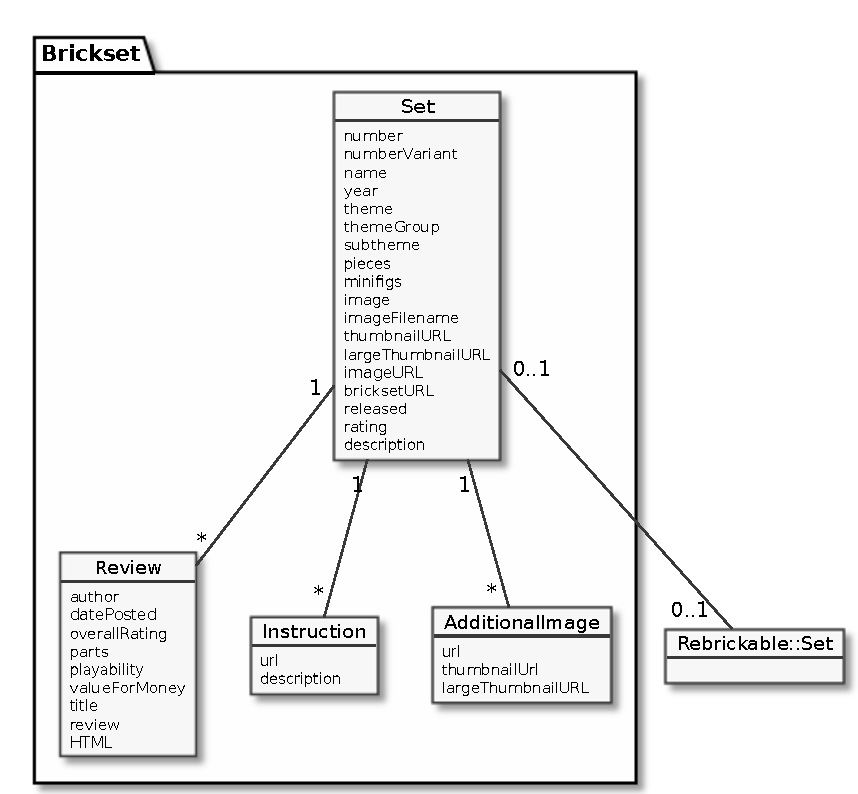
\includegraphics[width=\textwidth,height=\textheight,keepaspectratio]{pdfs/domain_brickset}
    \caption{Doménový model: Brickset \label{diagram-domenovy-brickset}}
\end{figure}